\documentclass[tikz,border=10pt]{standalone}
\usepackage{helvet}
\renewcommand{\familydefault}{\sfdefault}
\usepackage{tikz}
\usetikzlibrary{positioning, fit, calc, arrows.meta, shapes.geometric, backgrounds}

\definecolor{emeraldpine}{HTML}{1A4D3E}
\definecolor{harvardcrimson}{HTML}{A51C30}
\definecolor{ethdarkblue}{HTML}{1F407A}
\definecolor{ethpetrol}{HTML}{007A87}
\definecolor{ethbronze}{HTML}{B87333}
\definecolor{ethpurple}{HTML}{5B4B8A}
\definecolor{ink}{HTML}{1A202C}
\definecolor{softink}{HTML}{4A5568}
\definecolor{paleink}{HTML}{A0AEC0}
\definecolor{cardbg}{HTML}{F8FAFC}
\definecolor{shadecolor}{HTML}{F4F6F9}

\begin{document}
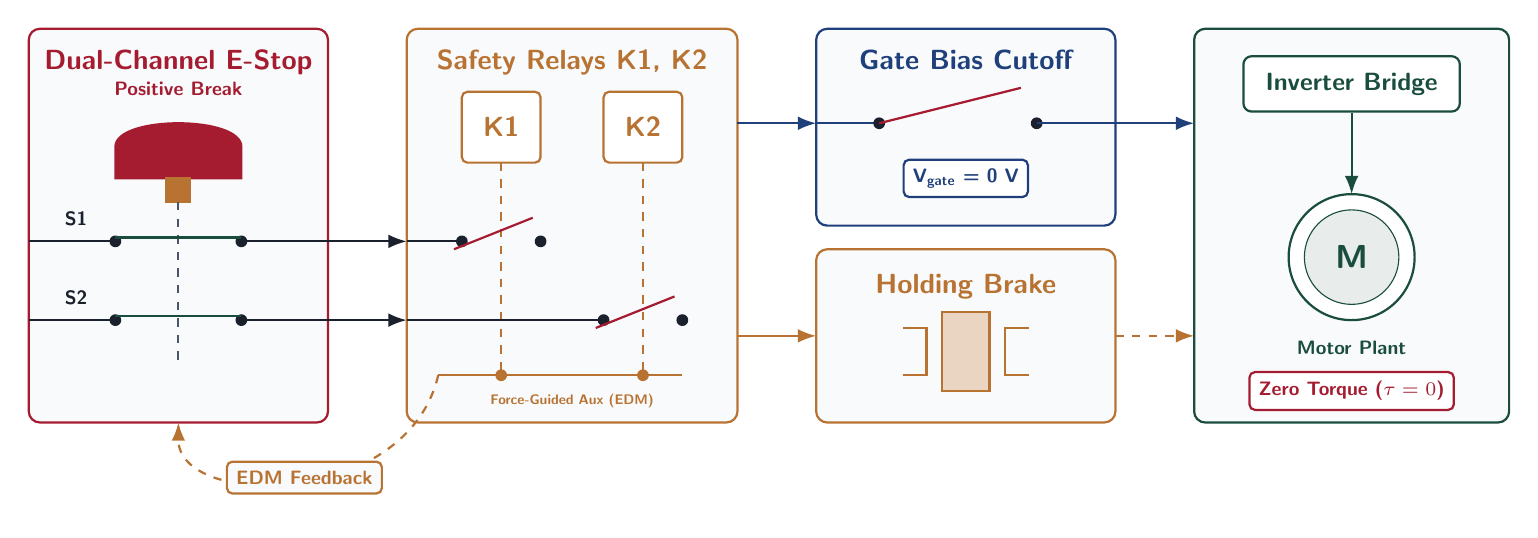
\begin{tikzpicture}[
    >=Latex,
    font=\sffamily,
    contact/.style={circle, fill=ink, inner sep=1.5pt},
    nc_switch/.style={thick, draw=emeraldpine},
    open_switch/.style={thick, draw=harvardcrimson},
    mech_link/.style={thick, dashed, draw=softink}
]

% STAGE 1: Dual-Channel E-Stop
\draw[draw=harvardcrimson, thick, rounded corners=4pt, fill=cardbg] (0,0) rectangle (3.8, 5);
\node[text=harvardcrimson, font=\bfseries, anchor=north] at (1.9, 4.85) {Dual-Channel E-Stop};
\node[text=harvardcrimson, font=\scriptsize\bfseries, anchor=north] at (1.9, 4.45) {Positive Break};

% E-stop button (adjusted lower for ample text clearance)
\draw[fill=harvardcrimson, draw=harvardcrimson, thick] (1.1, 3.1) -- (1.1, 3.5) .. controls (1.1, 3.9) and (2.7, 3.9) .. (2.7, 3.5) -- (2.7, 3.1) -- cycle;
\draw[fill=ethbronze, draw=ethbronze, thick] (1.75, 2.8) rectangle (2.05, 3.1);
\draw[mech_link] (1.9, 2.8) -- (1.9, 0.7);

% S1 Contact
\draw[thick, draw=ink] (0.0, 2.3) -- (1.1, 2.3);
\node[contact] (s1a) at (1.1, 2.3) {};
\node[contact] (s1b) at (2.7, 2.3) {};
\draw[nc_switch] (1.1, 2.35) -- (2.7, 2.35);
\draw[thick, draw=ink] (2.7, 2.3) -- (3.8, 2.3);
\node[anchor=south, font=\scriptsize\bfseries, text=ink] at (0.6, 2.38) {S1};

% S2 Contact
\draw[thick, draw=ink] (0.0, 1.3) -- (1.1, 1.3);
\node[contact] (s2a) at (1.1, 1.3) {};
\node[contact] (s2b) at (2.7, 1.3) {};
\draw[nc_switch] (1.1, 1.35) -- (2.7, 1.35);
\draw[thick, draw=ink] (2.7, 1.3) -- (3.8, 1.3);
\node[anchor=south, font=\scriptsize\bfseries, text=ink] at (0.6, 1.38) {S2};

% Wires to Stage 2
\draw[thick, ->, draw=ink] (3.8, 2.3) -- (4.8, 2.3);
\draw[thick, ->, draw=ink] (3.8, 1.3) -- (4.8, 1.3);

% STAGE 2: Safety Relays
\draw[draw=ethbronze, thick, rounded corners=4pt, fill=cardbg] (4.8,0) rectangle (9.0, 5);
\node[text=ethbronze, font=\bfseries, anchor=north] at (6.9, 4.85) {Safety Relays K1, K2};

% Relay Coils
\draw[thick, draw=ethbronze, fill=white, rounded corners=2pt] (5.5, 3.3) rectangle (6.5, 4.2);
\node[text=ethbronze, font=\bfseries] at (6.0, 3.75) {K1};
\draw[thick, draw=ethbronze, fill=white, rounded corners=2pt] (7.3, 3.3) rectangle (8.3, 4.2);
\node[text=ethbronze, font=\bfseries] at (7.8, 3.75) {K2};

% Linkages
\draw[mech_link, draw=ethbronze] (6.0, 3.3) -- (6.0, 0.6);
\draw[mech_link, draw=ethbronze] (7.8, 3.3) -- (7.8, 0.6);

% Contacts
\draw[thick, draw=ink] (4.8, 2.3) -- (5.5, 2.3);
\node[contact] (k1a) at (5.5, 2.3) {};
\node[contact] (k1b) at (6.5, 2.3) {};
\draw[open_switch] (5.4, 2.2) -- (6.4, 2.6); % Open

\draw[thick, draw=ink] (4.8, 1.3) -- (7.3, 1.3);
\node[contact] (k2a) at (7.3, 1.3) {};
\node[contact] (k2b) at (8.3, 1.3) {};
\draw[open_switch] (7.2, 1.2) -- (8.2, 1.6); % Open

% EDM Feedback contacts inside relay box
\draw[thick, draw=ethbronze] (5.2, 0.6) -- (8.3, 0.6);
\node[contact, fill=ethbronze] at (6.0, 0.6) {};
\node[contact, fill=ethbronze] at (7.8, 0.6) {};
\node[font=\tiny\bfseries, text=ethbronze, anchor=north] at (6.9, 0.48) {Force-Guided Aux (EDM)};

% EDM Feedback Loop back to Stage 1
\draw[thick, dashed, draw=ethbronze, ->] (5.2, 0.6) .. controls (4.8, -1.1) and (1.9, -1.1) .. (1.9, 0.0);
\node[fill=cardbg, draw=ethbronze, thick, rounded corners=2pt, text=ethbronze, font=\scriptsize\bfseries] at (3.5, -0.7) {EDM Feedback};

% Wires to Stage 3
\draw[thick, ->, draw=ethdarkblue] (9.0, 3.8) -- (10.0, 3.8);
\draw[thick, ->, draw=ethbronze] (9.0, 1.1) -- (10.0, 1.1);

% STAGE 3: Gate Bias Cutoff
\draw[draw=ethdarkblue, thick, rounded corners=4pt, fill=cardbg] (10.0, 2.5) rectangle (13.8, 5);
\node[text=ethdarkblue, font=\bfseries, anchor=north] at (11.9, 4.85) {Gate Bias Cutoff};

\draw[thick, draw=ethdarkblue] (10.0, 3.8) -- (10.8, 3.8);
\node[contact] (g1) at (10.8, 3.8) {};
\node[contact] (g2) at (12.8, 3.8) {};
\draw[open_switch] (10.8, 3.8) -- (12.6, 4.25);
\draw[thick, draw=ethdarkblue] (12.8, 3.8) -- (13.8, 3.8);

\node[fill=white, draw=ethdarkblue, thick, rounded corners=2pt, text=ethdarkblue, font=\scriptsize\bfseries] at (11.9, 3.1) {V\textsubscript{gate} = 0 V};

% STAGE 3: Holding Brake
\draw[draw=ethbronze, thick, rounded corners=4pt, fill=cardbg] (10.0, 0) rectangle (13.8, 2.2);
\node[text=ethbronze, font=\bfseries, anchor=north] at (11.9, 2.0) {Holding Brake};

% Brake icon
\draw[thick, draw=ethbronze] (11.1, 0.6) -- (11.4, 0.6) -- (11.4, 1.2) -- (11.1, 1.2);
\draw[thick, draw=ethbronze] (12.7, 0.6) -- (12.4, 0.6) -- (12.4, 1.2) -- (12.7, 1.2);
\draw[fill=ethbronze!30, draw=ethbronze, thick] (11.6, 0.4) rectangle (12.2, 1.4);

% Wires to Stage 4
\draw[thick, ->, draw=ethdarkblue] (13.8, 3.8) -- (14.8, 3.8);
\draw[thick, dashed, ->, draw=ethbronze] (13.8, 1.1) -- (14.8, 1.1);

% STAGE 4: Actuator / Inverter Bridge & Motor
\draw[draw=emeraldpine, thick, rounded corners=4pt, fill=cardbg] (14.8, 0) rectangle (18.8, 5);

% Inverter Box
\node[draw=emeraldpine, thick, fill=white, rounded corners=3pt, font=\bfseries\small, text=emeraldpine, inner xsep=8pt, inner ysep=6pt] (inv) at (16.8, 4.3) {Inverter Bridge};

\draw[thick, ->, draw=emeraldpine] (inv.south) -- (16.8, 2.9);

% Motor
\draw[thick, draw=emeraldpine, fill=white] (16.8, 2.1) circle (0.8);
\draw[draw=emeraldpine, fill=emeraldpine!10] (16.8, 2.1) circle (0.6);
\node[text=emeraldpine, font=\large\bfseries] at (16.8, 2.1) {M};
\node[text=emeraldpine, font=\scriptsize\bfseries] at (16.8, 0.95) {Motor Plant};

\node[fill=white, draw=harvardcrimson, thick, rounded corners=2pt, text=harvardcrimson, font=\scriptsize\bfseries] at (16.8, 0.4) {Zero Torque ($\tau = 0$)};

\end{tikzpicture}
\end{document}
